\documentclass[10pt,a4paper]{article}
\usepackage[utf8]{inputenc}
\usepackage[english]{babel}
\usepackage{amsmath}
\usepackage{amsfonts}
\usepackage{amssymb}
\usepackage{soul}
\usepackage[margin=1in]{geometry}
\usepackage{enumitem}
\usepackage{adjustbox}
\usepackage{multicol}
\usepackage{cancel}

\newlength{\drop}

\usepackage{tikz}

\newcommand{\inline}[2]{%
    \begin{tikzpicture}[baseline=(word.base), txt/.style={shape=rectangle, inner sep=0pt}]% the baseline key ensures that nodes won't shift up if there's text with descenders, and the txt style removes extra spacing so you can use this inline
    \node[txt] (word) {#1};% the first argument is the contents of the main node
    \node[above] at (word.north) {\footnotesize{#2}};% the second argument is the tag; you can play with the positioning as necessary
    \end{tikzpicture}%
    }

\begin{document}

\begin{titlepage}

\drop=0.1\textheight
    \centering
    \vspace*{\baselineskip}
    \rule{\textwidth}{1.6pt}\vspace*{-\baselineskip}\vspace*{2pt}
    \rule{\textwidth}{0.6pt}\\[\baselineskip]
    {\LARGE APUNTES DE\\[0.2\baselineskip] ROBOTICA}\\[0.2\baselineskip]
    \rule{\textwidth}{0.4pt}\vspace*{-\baselineskip}\vspace{3.2pt}
    \rule{\textwidth}{1.6pt}\\[\baselineskip]
    \scshape
    MODELO CINEMÁTICO DE VELOCIDAD \\
    \vspace*{2\baselineskip}
    %Edited by \\[\baselineskip]
    %{\Large MAXIMILIANO PONCE\par}
    %{\itshape My notes from \\Langpill english grammar course from Udemy, and Grammarly\\\par}
    \vfill
    {\scshape Abril 2020} \\
    {\large MAXIMILIANO PONCE}\par

\end{titlepage}

\tableofcontents
\newpage

\section{Modelo cinemático de velocidad}
En esta sección se derivan las relaciones de velocidad, con respecto a las velocidades lineales y angulares del efector final. Las relaciones de velocidad se determinan por los Jacobianos de la cinemática directa.\\

Velocidad angular: Caso de eje fijo\\

\begin{figure}[h]
     \centering
     \begin{center}
		 $\omega = \dot{\theta} \vec{k}$ \\
     	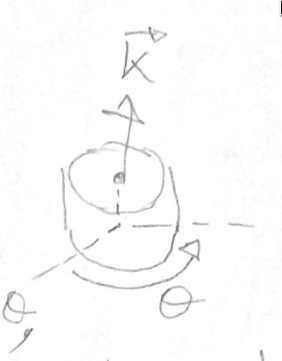
\includegraphics[width=0.2\linewidth]{f1}
     \end{center}
\end{figure}


donde $\dot{\theta}$ es la derivada con respecto al tiempo de $\theta$, $\vec{k}$ es un vector en dirección del eje de rotación y $\omega$ es la velocidad angular. Dada la velocidad angular del cuerpo, la velocidad lineal de cualquier punto en el cuerpo esta dada por:

$$ \upsilon = \omega \times \vec{r}$$

donde $\vec{r}$ es un vector desde el origen al punto dado. La velocidad angular $\omega$ es una propiedad de la trama anexa al cuerpo. La velocidad angular no es una propiedad de un punto particular. Asi que $\upsilon$ corresponde a la velocidad lineal de un punto mientras $\omega$ corresponde a la velocidad angular de una trama rotando.

\subsection{Matrices asimétricas}
Se dice que una matriz $S$ es asimétrica si y sólo si:
$$ S^T + S = 0$$

donde,
$$
	S =
	\begin{bmatrix}
		0    & -s_3 & s_2\\
		s_3  & 0    & -s_1\\
		-s_2 & s_1  & 0
	\end{bmatrix}
$$

\textbf{Por ejemplo}: si se definen a los tres vectores unitarios de un sistema de coordenadas como $\vec{i}$, $\vec{j}$, $\vec{k}$, representados como:
$$
	\vec{i} =
	\begin{bmatrix}
		1 \\ 0 \\ 0
	\end{bmatrix},
	\vec{j} =
	\begin{bmatrix}
		0 \\ 1 \\ 0
	\end{bmatrix},
	\vec{k} =
	\begin{bmatrix}
		0 \\ 0 \\ 1
	\end{bmatrix}
$$

Entonces las matrices asimétricas $S(\vec{i}), S(\vec{j}), S(\vec{k})$ se definen como:

$$
	S(\vec{i}) =
	\begin{bmatrix}
		0 & 0 & 0 \\
		0 & 0 & -1\\
		0 & 1 & 0
	\end{bmatrix},
	S(\vec{j}) =
	\begin{bmatrix}
		0 & 0 & 1 \\
		0 & 0 & 0\\
		-1& 0 & 0
	\end{bmatrix},
	S(\vec{k}) =
	\begin{bmatrix}
		0 & -1 & 0 \\
		1 & 0 & 0\\
		0 & 0 & 0
	\end{bmatrix}
$$

Derivada de una matriz de rotación:

$$
	R(\theta) \cdot R(\theta)^T=I
$$

Obteniendo la derivada de la ecuación anterior se tiene:


$$
	\frac{dR}{d\theta} \cdot R(\theta)^T + R(\theta) \cdot \frac{dR^T}{d\theta} = 0
$$

\begin{multicols}{2}

	Se define a $S$ como,

	$$ S:=\frac{dR}{d\theta} \cdot R(\theta)^T $$

	entonces, la transpuesta de $S$ es,

	$$ S^T = \left( \frac{dR}{d\theta} \cdot R(\theta)^T \right)^T = R(\theta) \cdot \frac{dR^T}{d\theta} $$

	Por lo que se cumple

	$$ S + S^T = 0$$

	\columnbreak
	\fbox{\begin{minipage}{15em}
	\textbf{Demostración} \\
	$$ S = \frac{dR}{d\theta} \cdot R(\theta)^T $$
	$$ \frac{dR}{d\theta} = \frac{S}{R(\theta)^T} $$
	$$ R(\theta)^T = R(\theta)^{-1} = \frac{1}{R(\theta)} $$
	$$ \frac{dR}{d\theta} = \frac{S}{ \frac{1}{R(\theta)} } $$
	$$ \frac{dR}{d\theta} = S \cdot R(\theta) $$
	\end{minipage}}
\end{multicols}

En otras palabras la matriz $S$ es una matriz asimétrica. Entonces,

$$ S \cdot R(\theta) = \frac{dR}{d\theta} R(\theta) R(\theta)^T $$

\[
	\boxed{\frac{dR}{d\theta} = S R(\theta)} \quad \dot{R}(\theta) = S R(\theta)
 \]

\vspace{0.5cm}

 \textbf{Ejemplo:} Si $R=R_{\vec{x},\theta}$ donde  $R_{\vec{x}}$ se refiere a la matriz de rotación básica que se gira sobre el eje $x$, entonces

 $$
	S = \frac{dR}{d\theta} R^T = \frac{d}{d\theta}
	\begin{Bmatrix}
	\begin{bmatrix}
		1 & 0 & 0 \\
		0 & c\theta & -s\theta\\
		0 & s\theta & c\theta
	 \end{bmatrix}
	 \end{Bmatrix}
	\cdot
	 \begin{bmatrix}
	 	1 & 0 & 0 \\
		0 & c\theta & -s\theta\\
		0 & s\theta & c\theta
	 \end{bmatrix}^T =
	\begin{bmatrix}
	 	0 & 0 & 0 \\
		0 & -s\theta & -c\theta\\
		0 & c\theta & -s\theta
	 \end{bmatrix} \cdot
	 \begin{bmatrix}
	 	1 & 0 & 0 \\
		0 & c\theta & s\theta\\
		0 & -s\theta & c\theta
	 \end{bmatrix}
 $$

 $$
	S =
	\begin{bmatrix}
		0 & 0 & 0 \\
		0 & \cancel{-s\theta c\theta + s\theta c\theta} & -s^2\theta - c^2\theta \\
		0 & c^2\theta + s^2\theta & \cancel{s\theta c\theta - s\theta c\theta}
	\end{bmatrix} =
	\begin{bmatrix}
		0 & 0 & 0 \\
		0 & 0 & -1 \\
		0 & 1 & 0
	\end{bmatrix} = S(i)
 $$

\end{document}
